\documentclass[french,onlymath]{beamer}

%%%%%%%%%%%%%%%%%%%%%%%%%%%%%%%%%%%%%%%%%%%%%%%%%%%%%%%%%%%%%%%%%%%%%%%%%%%%%%
\input{preambule_presentation_2013_2014}
%___________________________
%===   Redéfinition des marges par défaut
%------------------------------------------------------
%\usepackage[textwidth=18.6cm]{geometry}%à mettre dans le preambule perso
%\pagestyle{fancy}%à mettre dans le preambule perso


\setlength\paperheight{297mm}
\setlength\paperwidth{210mm}
\setlength{\evensidemargin}{0cm}% Marge gauche sur pages paires
\setlength{\oddsidemargin}%{0cm}%
{-0.5cm}% Marge gauche sur pages impaires
\setlength{\topmargin}{-2cm}% Marge en haut
\setlength{\headsep}{0.5cm}% Entre le haut de page et le texte
\setlength{\headheight}{0.7cm}% Haut de page
\setlength{\textheight}{25.2cm}% Hauteur de la zone de texte
\setlength{\textwidth}{17cm}% Largeur de la zone de texte


% Environnement enumerate
\renewcommand{\theenumi}{\bf\textsf{\arabic{enumi}}}
\renewcommand{\labelenumi}{\bf\textsf{\theenumi.}}
\renewcommand{\theenumii}{\bf\textsf{\alph{enumii}}}
\renewcommand{\labelenumii}{\bf\textsf{\theenumii.}}
\renewcommand{\theenumiii}{\bf\textsf{\roman{enumiii}}}
\renewcommand{\labelenumiii}{\bf\textsf{\theenumiii.}}


\usetikzlibrary{shadows,trees}


%definition des couleurs
\definecolor{fondpaille}{cmyk}{0,0,0.1,0}%\pagecolor{fondpaille}
\definecolor{gris}{rgb}{0.7,0.7,0.7}
\definecolor{rouge}{rgb}{1,0,0}
\definecolor{bleu}{rgb}{0,0,1}
\definecolor{vert}{rgb}{0,1,0}
\definecolor{deficolor}{HTML}{2D9AFF}
\definecolor{backdeficolor}{HTML}{EDEDED}%{036DD0}%dégradé bleu{666666}%dégradé gris
\definecolor{theocolor}{HTML}{036DD0}%F4404D%rouge
\definecolor{backtheocolor}{HTML}{D3D3D3}
\definecolor{methcolor}{HTML}{008800}%12BB05}
\definecolor{backmethcolor}{HTML}{FFFACD}
\definecolor{backilluscolor}{HTML}{EDEDED}
\definecolor{sectioncolor}{HTML}{B2B2B2}%vert : {HTML}{008800}%{HTML}{2D9AFF}
\definecolor{subsectioncolor}{HTML}{B2B2B2}%vert : {HTML}{008800}%{rgb}{0.5,0,0}
\definecolor{engcolor}{HTML}{D4D7FE}
\definecolor{exocolor}{rgb}{0,0.6,0}
\definecolor{exosoltitlecolor}{rgb}{0,0.6,0}
\definecolor{titlecolor}{rgb}{1,1,1}

%commande pour enlever les couleurs avant impression
\newcommand{\nocolor}
{\pagecolor{white}
\definecolor{gris}{rgb}{0.7,0.7,0.7}
\definecolor{rouge}{rgb}{0,0,0}
\definecolor{bleu}{rgb}{0,0,0}
\definecolor{vert}{rgb}{0,0,0}
\definecolor{deficolor}{HTML}{B2B2B2}
\definecolor{backdeficolor}{HTML}{EEEEEE}%{036DD0}%dégradé bleu{666666}%dégradé gris
\definecolor{theocolor}{HTML}{B2B2B2}
\definecolor{backtheocolor}{HTML}{EEEEEE}
\definecolor{methcolor}{HTML}{B2B2B2}
\definecolor{backmethcolor}{HTML}{EEEEEE}
\definecolor{backilluscolor}{HTML}{EEEEEE}
\definecolor{sectioncolor}{HTML}{B2B2B2}
\definecolor{subsectioncolor}{HTML}{B2B2B2}
\definecolor{engcolor}{HTML}{EEEEEE}
\definecolor{exocolor}{HTML}{3B3838}
\definecolor{exosoltitlecolor}{rgb}{0,0,0}
\definecolor{titlecolor}{rgb}{0,0,0}
}



%___________________________
%===    Exercice résolu
%------------------------------------------------------
%
%#1 : énoncé
%#2 : solution
\newcounter{exosol}
\newcommand{\exosol}[2]{
\stepcounter{exosol}
\begin{tikzpicture}[node distance=0 cm]
\node[fill=backilluscolor,rounded corners=2pt,anchor=south west] (illus) at (0,-0.02)
{\it \textbf{\textcolor{exosoltitlecolor}{Exercice résolu \arabic{exosol}~:~}}};
\node[fill=backilluscolor,rounded corners=2pt,anchor=north west]at(0,0)
{\parbox{\columnwidth-10pt}{#1\par\medskip{\it \textbf{\textcolor{exosoltitlecolor}{Solution~:~}}}\par#2 }};
\end{tikzpicture}
\bigskip
}

\newcommand{\suite}[1]{
\begin{tikzpicture}[node distance=0 cm]
\node[fill=backilluscolor,rounded corners=2pt,anchor=north west]at(0,0)
{\parbox{\columnwidth-10pt}{{\it \textbf{\textcolor{exosoltitlecolor}{Suite de la solution~:}}}\par#1}};
\end{tikzpicture}
\bigskip
}



%%%%%%%%%%%%%%%%%%%%%%%%%%%%%%%%%%%%%%%%%%%%%%%%%%%%%%%%%%%%%%%%%%%%%%%%%%%%%%%
%Encadrés pour Propriétés, Théorème, Définitions, exemples, exercices

\usepackage{environ}%pour pouvoir utiliser la commande \NewEnviron

%___________________________
%===    Propriété avec ou sans s et avec ou sans titre
%------------------------------------------------------
%
\NewEnviron{Prop}[2][]{
\begin{tikzpicture}[node distance=0 cm]
\node[fill=theocolor,rounded corners=5pt,anchor=south west] (theorem) at (0,0)
{\textcolor{titlecolor}{Propriété#1~:~#2}};
\node[draw,drop shadow,color=theocolor,very thick,fill=backtheocolor,rounded corners=5pt,anchor=north west] at(0,-0.02)
{\black\parbox{\columnwidth-12pt}{\BODY}};
\end{tikzpicture}
\bigskip
}


%___________________________
%===    Théorème avec ou sans titre
%------------------------------------------------------
%
\NewEnviron{Thm}[1][]{
\begin{tikzpicture}[node distance=0 cm]
\node[fill=theocolor,rounded corners=5pt,anchor=south west] (theorem) at (0,0)
{\textcolor{titlecolor}{Théorème~:~#1}};
\node[draw,drop shadow,color=theocolor,very thick,fill=backtheocolor,rounded corners=5pt,anchor=north west] at(0,-0.02)
{\black\parbox{\columnwidth-12pt}{\BODY}};
\end{tikzpicture}
\medskip
}



%___________________________
%===    Définition avec ou sans s et avec sans titre
%------------------------------------------------------
%
\NewEnviron{Defi}[2][]{
\begin{tikzpicture}[node distance=0 cm]
\node[fill=theocolor,rounded corners=5pt,anchor=south west] (theorem) at (0,0)
{\textcolor{titlecolor}{Définition#1~:~#2}};
\node[draw,drop shadow,color=deficolor,very thick,fill=backdeficolor,rounded corners=5pt,anchor=north west] at(0,-0.02)
{\black\parbox{\columnwidth-12pt}{\BODY}};
\end{tikzpicture}
\medskip
}

%___________________________
%===    Méthode avec ou sans s et avec sans titre
%------------------------------------------------------
%
\NewEnviron{Methode}[2][]{
\begin{tikzpicture}[node distance=0 cm]
\node[fill=theocolor,rounded corners=5pt,anchor=south west] (theorem) at (0,0)
{\textcolor{titlecolor}{Méthode#1~:~#2}};
\node[draw,drop shadow,color=methcolor,very thick,fill=backmethcolor,rounded corners=5pt,anchor=north west] at(0,-0.02)
{\black\parbox{\columnwidth-12pt}{\BODY}};
\end{tikzpicture}
\medskip
}


%___________________________
%===    Redéfinition de la commande \chapter{•}
%------------------------------------------------------
%
\makeatletter

\renewcommand{\@makechapterhead}[1]{
\begin{tikzpicture}
\node[fill=theocolor,rectangle,rounded corners=5pt]{%
\begin{minipage}{\linewidth}
\begin{center}
\vspace*{9pt}
\textcolor{titlecolor}{\Large \textsc{\textbf{Chapitre \thechapter \ : \ #1}}}
\vspace*{9pt}
\end{center}
\end{minipage}
};\end{tikzpicture}
}

\makeatother


%___________________________
%===    Exemple avec ou sans s et avec ou sans titre
%------------------------------------------------------
%
\NewEnviron{Exemple}[2][]{
\begin{tikzpicture}[node distance=0 cm]
\node[draw,drop shadow,color=methcolor,very thick,fill=backmethcolor,rounded corners=5pt,anchor=north west] at(0,-0.02)
{\black\parbox{\columnwidth-12pt}{\textbf{Exemple#1~:~#2}\\
\BODY}};
\end{tikzpicture}
\medskip
}

%___________________________
%===    Remarque avec ou sans s
%------------------------------------------------------
%
\NewEnviron{Rmq}[1][]{
\textbf{\large{Remarque#1 :}}\par
\BODY
\medskip
}

%___________________________
%===    Remarques numérotées R1, R2, etc...
%------------------------------------------------------
%
\newcounter{rem}\newcommand{\rem}{\refstepcounter{rem}\textbf{R \therem \ :}\xspace}

%___________________________
%===    Exercices du contrôle numérotés
%------------------------------------------------------
%
\newcounter{exercice}
\NewEnviron{Exercice}[1][]{
\refstepcounter{exercice}\textbf{\large{Exercice \theexercice \ :}}\hfill \textbf{#1}\par
\BODY
\medskip
}

%___________________________
%===    Exercices non numérotés
%------------------------------------------------------
%
\NewEnviron{Exo}[1][]{
\textbf{\large{Exercice #1 \ :}}\par
\BODY
\medskip
}

%___________________________
%===    Démonstration
%------------------------------------------------------
\NewEnviron{Demo}{%
\textit{\textbf{Démonstration.}}\par
\BODY
\strut\hfill$\square$
\medskip
}

%___________________________
%===    Commandes perso
%------------------------------------------------------
%
%\Leftrightarrow
\newcommand{\Lr}{\Leftrightarrow}

%Ancienne commande chapitre
\newcommand{\chapitre}[1]{
\begin{tikzpicture}
\node[fill=theocolor,rectangle,rounded corners=5pt]{%
\begin{minipage}{\linewidth}
\begin{center}
\vspace*{9pt}
\textcolor{titlecolor}{\Large \textsc{\textbf{#1}}}
\vspace*{9pt}
\end{center}
\end{minipage}
};
\end{tikzpicture}
\bigskip
}

%Pour les fiches : commande de Cécile
\newcommand{\Fiche}[2]{%
\begin{tikzpicture}
	\node[draw, color=blue,fill=white,rectangle,rounded corners=5pt]{%
	\begin{minipage}{\linewidth}
		\begin{center}
			\vspace*{9pt}
			\textcolor{blue}{\Large \textsc{\textbf{Fiche~#1\ :\ #2}}}
			\vspace*{7pt}
		\end{center}
	\end{minipage}
	};
\end{tikzpicture}
}%

\pagecolor{white}%couleur du fond de page

\renewcommand{\Pointilles}{%
\makebox[\linewidth]{\dotfill}
}



%%%%%%%%%%%%%%%%%%%%%%%%%%%%%%%%%%%%%%%%%%%%%%%%%%%%%%%%%%%%%%%%%%%%%%%%%%%%%%%
%%%%%%%%%%%%%%%%%%%%%%%%%%%%%%%%%%%%%%%%%%%%%%%%%%%%%%%%%%%%%%%%%%%%%%%%%%%%%%
%Titre présentation Beamer
\title{Correction de l'exercice supplémentaire n° 1}  
\author{BAT 2}\institute{Lycée Jean Pierre Timbaud}
\date{}
%%%%%%%%%%%%%%%%%%%%%%%%%%%%%%%%%%%%%%%%%%%%%%%%%%%%%%%%%%%%%%%%%%%%%%%%%%%%%%%%%

%%%%%%%%%%%%%%%%%%%%%%%
%% DEBUT DU DOCUMENT %%
%%%%%%%%%%%%%%%%%%%%%%%

\begin{document}



%%%%%%%%%%%%%%%%%%%%%%%Page 1%%%%%%%%%%%%%%%%%%%%%%%%%%%%%%%%%%%%%%%%
%\begin{spacing}{1.2}

%%%%%%%%%%%%%%%%%%%%%%%%%%%%%%%%%%%%%%%%%%%%%%%%%%%%%%%%%%%%
\begin{frame}
 \titlepage
\end{frame}
%%%%%%%%%%%%%%%%%%%%%%%%%%%%%%%%%%%%%%%%%%%%%%%%%%%%%%%%%%%%%
\section{Question a)}
\begin{frame}{Question a)}

\begin{itemize}
 	
	\item Je n'ai pas le même énoncé que vous...
	
	\item Dans mon livre, la question porte sur l'année 2006.
	
	\item Notons $(u_n)$ la production de bicyclettes pour la consommation intérieure à l'année $2005+n$ (ce qui signifie que $u_0=2 000 000$) et $(v_n)$ la production pour l'exportation à la même année ($v_0=250 000$).
	
	\item Notons $(w_n)$ la production totale de bicyclette à l'année $2005+n$.
	
	\item On a donc, pour tout $n \in \N$, $w_n=u_n+v_n$.
	
	\item $u_1=2 000 000 \times 1,1 = 2 200 000$, $v_1=250 000 \times 1,32 = 330 000$.
	
	\item Donc, la production totale pour 2006 doit être de :
	
	\item $w_1=u_1+v_1=2 200 000+330 000=2 530 000$ bicyclettes.
	
	\end{itemize}
\end{frame}


%%%%%%%%%%%%%%%%%%%%%%%%%%%%%%%%%%%%%%%%%%%%%%%%%%%%%%%%%%%%%%%%%
\section{Question b)}

\begin{frame}[allowframebreaks]{Question b)}


\label{départ}

\pause
\begin{block}{Un bloc normal}
On cherche $w_8=u_8+v_8$.
\end{block}	

\pause	
\setbeamertemplate{blocks}[rounded]
[shadow=true]	
	\begin{block}{Un bloc ombré}
On cherche $w_8=u_8+v_8$.
\end{block}

\begin{itemize}		
	\item La suite $(u_n)$ est la suite géométrique de premier terme $u_0=2 000 000$ et de raison $b=1,1$.
		
	\item La suite $(v_n)$ est la suite géométrique de premier terme $v_0=250 000$ et de raison $b=1,32$.
	
	\item Ainsi, pour tout $n \in \N$, on a :
	
	\item $u_n=u_0 \times a^n=2 000 000 \times 1,1^n$ et $v_n=v_0 \times b^n=250 000 \times 1,32^n$.
	
	\item Donc, $w_8=u_8+v_8=2 000 000 \times 1,1^8 + 250 000 \times 1,32^8 \approx 6 591 438$.
	
	\item Pour satisfaire la demande, la production devra être de 6 591 438 bicyclettes en 2013.
	
	\item\textcolor{orange}{Si on utilise la fonction $\ln$ pour résoudre l'inéquation (*), on écrira :}
		
	\pause\item\textcolor{orange}{$1,2^n > 8 \Leftrightarrow \ln \left( 1,2^n\right) > \ln (8) \Leftrightarrow n \ln (1,2) > \ln (8)$\\
	$\Leftrightarrow n > \dfrac{\ln(8)}{\ln(1,2)}$}
		
	\pause\item\textcolor{orange}{Or $\dfrac{\ln(8)}{\ln(1,2)} \approx 11,4$.}
	
	\pause\item\textcolor{orange}{On obtient donc la même conclusion.}
	
	\end{itemize}
\end{frame}


%%%%%%%%%%%%%%%%%%%%%%%%%%%%%%%%%%%%%%%%%%%%%%%%%%%%%%%%%%%%%

\section{Question c)}

\begin{frame}{Question c)}

\begin{itemize}
 	
	\item On cherche $n$ pour que $v_n > u_n$, c'est-à-dire
		
	\item $250 000 \times 1,32^n > 2 000 000 \times 1,1^n$.
		
	\item Or, $250 000 \times 1,32^n > 2 000 000 \times 1,1^n$\\ $\Leftrightarrow \dfrac{1,32^n}{1,1^n} > \dfrac{2 000 000}{250 000} \Leftrightarrow \left( \dfrac{1,32}{1,1}\right)^n > 8 \Leftrightarrow 1,2^n > 8$. (*)
	
	\item Nous n'avons pas, pour l'instant, de formule permettant de trouver l'entier $n$ qui convient.
	
	\item En essayant quelques valeurs de $n$, on obtient :
	
	\item $1,2^{11} \approx 7,4$ et $1,2^{12} \approx 8,9$.
	
	\item C'est donc à partir de la $12^{\text{ème}}$ année (après 2005, c'est-à-dire en 2017) que l'exportation dépassera pour la première fois la consommation intérieure.
	
	\end{itemize}
\end{frame}


%%%%%%%%%%%%%%%%%%%%%%%%%%%%%%%%%%%%%%%%%%%%%%%%%%%%%%%%%%%%%

\section{Avec la fonction ln}



\begin{frame}
%:-+-+-+-+- Engendré par : http://math.et.info.free.fr/TikZ/TableauxVariations/
\begin{center}
\begin{tikzpicture}[scale=0.875]
% Styles 
\tikzstyle{cadre}=[thin]
\tikzstyle{fleche}=[->,>=latex,thin]
\tikzstyle{nondefini}=[lightgray]
% Dimensions Modifiables
\def\Lrg{1.5}
\def\HtX{1}
\def\HtY{0.5}
% Dimensions Calculées
\def\lignex{-0.5*\HtX}
\def\lignef{-1.5*\HtX}
\def\separateur{-0.5*\Lrg}
% Largeur du tableau
\def\gauche{-1.5*\Lrg}
\def\droite{4.5*\Lrg}
% Hauteur du tableau
\def\haut{0.5*\HtX}
\def\bas{-2.5*\HtX-2*\HtY}
% Ligne de l'abscisse : x
\node at (-1*\Lrg,0) {$x$};
\node at (0*\Lrg,0) {$-\infty$};
\node at (2*\Lrg,0) {$0$};
\node at (4*\Lrg,0) {$+\infty$};
% Ligne de la dérivée : f'(x)
\node at (-1*\Lrg,-1*\HtX) {$f'(x)$};
\node at (0*\Lrg,-1*\HtX) {$$};
\node at (1*\Lrg,-1*\HtX) {$-$};
\node at (2*\Lrg,-1*\HtX) {$$};
\node at (3*\Lrg,-1*\HtX) {$+$};
\node at (4*\Lrg,-1*\HtX) {$$};
% Ligne de la fonction : f(x)
\node  at (-1*\Lrg,{-2*\HtX+(-1)*\HtY}) {$f$};
\node (f1) at (0*\Lrg,{-2*\HtX+(0)*\HtY}) {$+\infty$};
\node (f2) at (2*\Lrg,{-2*\HtX+(-2)*\HtY}) {$0$};
\node (f3) at (4*\Lrg,{-2*\HtX+(0)*\HtY}) {$+\infty$};
% Flèches
\draw[fleche] (f1) -- (f2);
\draw[fleche] (f2) -- (f3);
% Encadrement
\draw[cadre] (\separateur,\haut) -- (\separateur,\bas);
\draw[cadre] (\gauche,\haut) rectangle  (\droite,\bas);
\draw[cadre] (\gauche,\lignex) -- (\droite,\lignex);
\draw[cadre] (\gauche,\lignef) -- (\droite,\lignef);
\end{tikzpicture}
\end{center}
%:-+-+-+-+- Fin

%:>>>>> code du tableau à ré-injecter
%[
%	["x", "f'(x)", "Variatiosn \\par de \\par f"],
%	["-\\infty", "", "-", "+\\infty"],
%	["0", "", "+", "0"],
%	["+\\infty", "", "?", "+\\infty"]
%]

\end{frame}

\begin{frame}
\begin{minipage}{0.45\linewidth}
bonjour

\includegraphics[width=0.3\textwidth]{fig1}
\end{minipage}
\hspace{0.05\linewidth}
\begin{minipage}{0.45\linewidth}
au revoir

\hyperlink{départ}{\beamerskipbutton{Départ}}

\href{run:geogebra.ggb}{\beamerskipbutton{Ficher Geogebra}}

\includegraphics[width=0.3\textwidth]{fig1}
\end{minipage}
\end{frame}

%%%%%%%%%%%%%%%%%%%%%%%%%%%%%%%%%%%%%%%%%%%%%%%%%%%%%%%%%%%%
%\setenumerate{font=\color{blue} \bfseries} à insérer dans le préambule pour l'appliquer à tout le document


\begin{frame}{\'Equations de droites}
%On considère le repère suivant dans lequel on a placé quatre points.\\[6pt]
\begin{minipage}{0.6\linewidth}
\begin{tikzpicture}[scale=0.45,line cap=round,line join=round,>=stealth,x=1.0cm,y=1.0cm]
\draw [color=gray!, xstep=1,ystep=1,line width=1.5pt] (-6.5,-5.5) grid (8.5,5.5);
\draw[->,line width=1.5pt,color=blue] (-6.5,0) -- (8.5,0);
\foreach \x in {-6,...,8}
\draw[color=black] (\x,2pt) -- (\x,-2pt) node[below,font=\bfseries] {\x};
\draw[->,line width=1.5pt,color=blue] (0,-5.5) -- (0,5.5);
\foreach \y in {-5,...,5}
\draw[color=black] (2pt,\y) -- (-2pt,\y) node[left,font=\bfseries] {\y};
\clip(-6.5,-5.5) rectangle (8.5,5.5);%%%%%%%%%%%%réduit la fenêtre d'affichage de ce qui suit
\draw (-2,3) node [below left,font=\bfseries] {A};
\draw [line width=1.5pt] (-2,3)-- ++(3pt,3pt)-- ++(-6pt,-6pt)-- ++(3pt,3pt)-- ++(-3pt,3pt)-- ++(6pt,-6pt);
\draw (2,-1) node [below left,font=\bfseries] {B};
\draw [line width=1.5pt] (2,-1)-- ++(3pt,3pt)-- ++(-6pt,-6pt)-- ++(3pt,3pt)-- ++(-3pt,3pt)-- ++(6pt,-6pt);
\draw (1,4) node [below left,font=\bfseries] {C};
\draw [line width=1.5pt] (1,4)-- ++(3pt,3pt)-- ++(-6pt,-6pt)-- ++(3pt,3pt)-- ++(-3pt,3pt)-- ++(6pt,-6pt);
\draw (6,-4) node [below left,font=\bfseries] {D};
\draw [line width=1.5pt] (6,-4)-- ++(3pt,3pt)-- ++(-6pt,-6pt)-- ++(3pt,3pt)-- ++(-3pt,3pt)-- ++(6pt,-6pt);
\end{tikzpicture}
\end{minipage}
\hfill
\begin{minipage}{0.35\linewidth}
\pause
\begin{enumerate}[label=\arabic*.,font=\color{blue} \bfseries]
\item Donner les coordonnées des quatre points.
\pause
\item Déterminer une équation de la droite $(AC)$.
\pause
\item 	\begin{enumerate}[label=\alph*),font=\color{blue} \bfseries]
	\item Tracer la droite d'équation 
	
	$y=-2x-1$.

	\end{enumerate}

\end{enumerate}

\end{minipage}
\pause 
	\begin{enumerate}[label=\alph*),start=2,leftmargin=1.5cm,font=\color{blue} \bfseries]
	\item Par quel point déjà sur le graphique semble-t-elle passer ?
\pause	
	\item Vérifier par le calcul la réponse à la question précédente.
	\end{enumerate}
\pause
\begin{enumerate}[label=\arabic*.,resume,font=\color{blue} \bfseries]
\item Déterminer par le calcul si les points $A$, $B$ et $C$ sont alignés ou non.

\end{enumerate}

\end{frame}
%%%%%%%%%%%%%%%%%%%%%%%%%%%%%%%%%%%%%%%%%%%%%%%%%%%%%%%%%%%%

%\end{spacing}

%%%%%%%%%%%%%%%%%%%%%%%%%%%%%%%%%%%%%%%%%%%%%%%%%%%%%%%%%%%%
%%%%%%%%%%%%%%%%%%%%%
%% FIN DU DOCUMENT %%
%%%%%%%%%%%%%%%%%%%%%
\end{document}